\subsection*{Диграмма последовательностей}

UML диаграмма последовательности (Sequence diagram) - это диаграмма, которая отображает взаимодействие между объектами или компонентами в системе
в виде последовательности сообщений, которые передаются между ними.

Диаграмма последовательностей спроектирована в draw.io \cite{drawio} и изображена на рис.~\ref{fig:UML_sequence_diagram}.

UML диаграмма последовательности позволяет представить взаимодействие между объектами в форме временной последовательности,
показывая, как каждый объект взаимодействует с другими и когда это происходит. Объекты изображаются в виде вертикальных линий (жизненных линий),
а сообщения между объектами отображаются в виде стрелок, которые указывают направление передачи информации.

\begin{figure}[!htb]
    \centering

    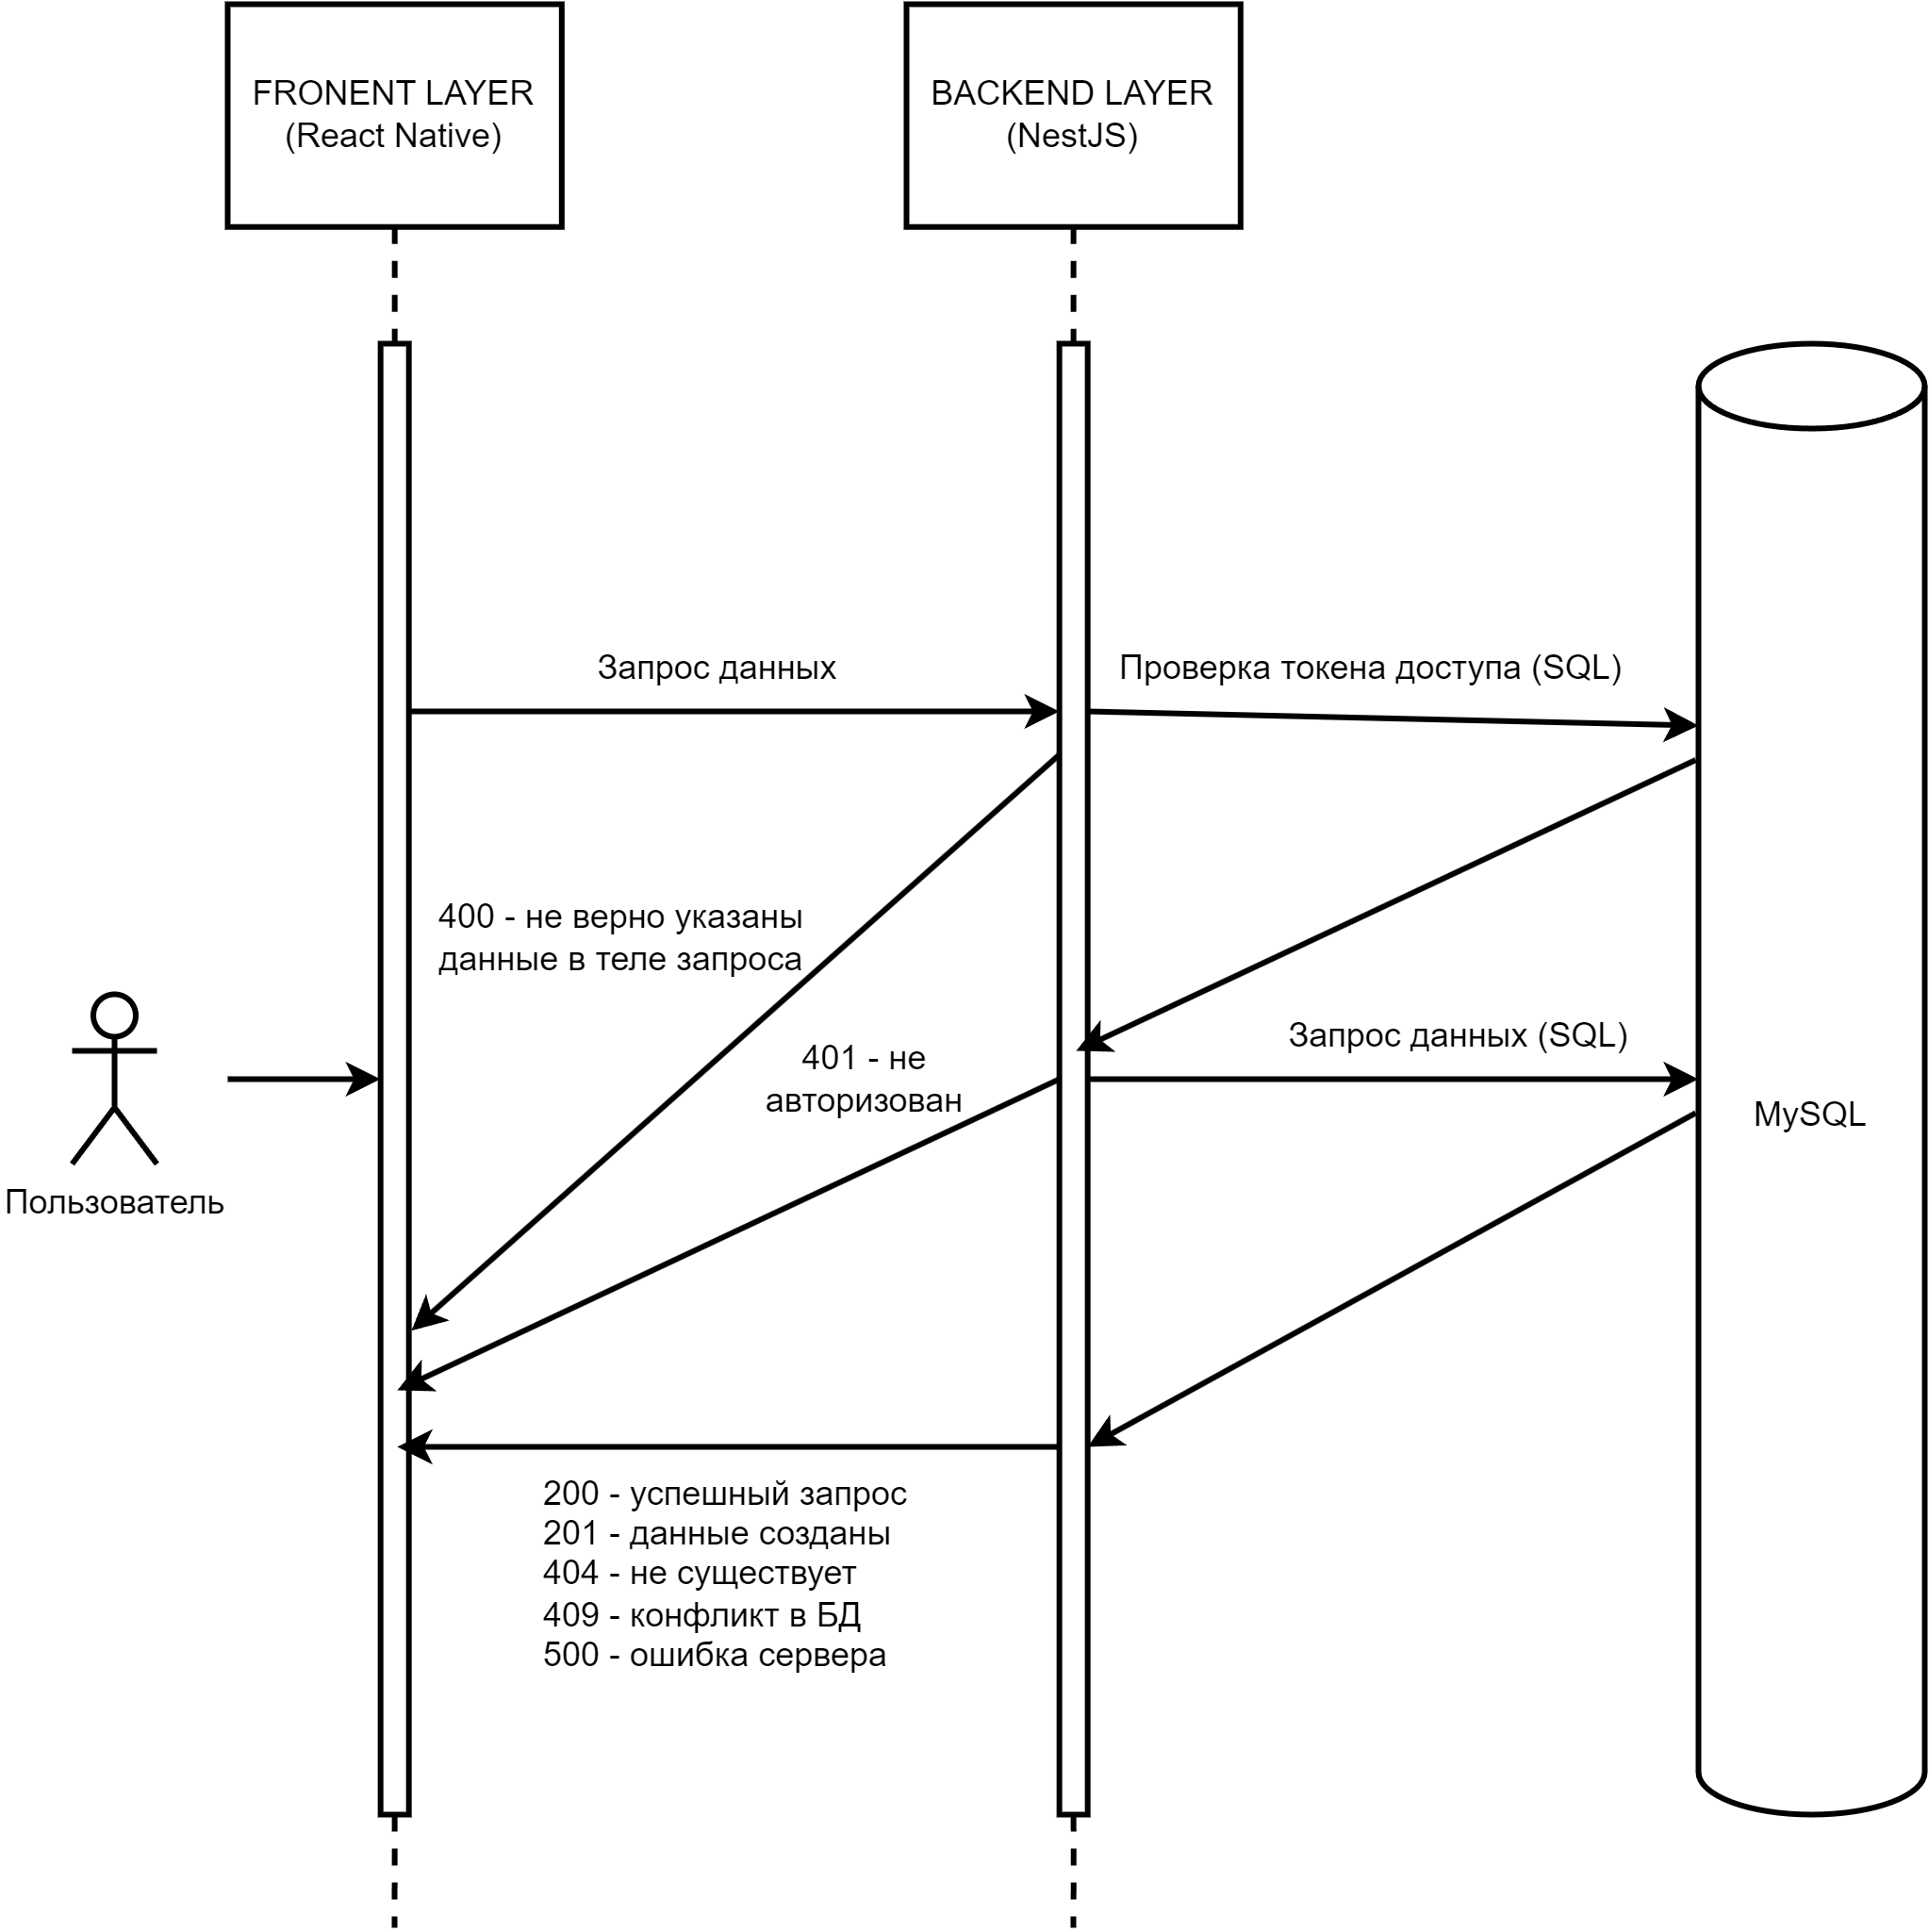
\includegraphics[width=16cm]
    {images/UML/UML_sequence_diagram.png}

    \caption{Диаграмма последовательностей}

    \label{fig:UML_sequence_diagram}
\end{figure}
